O modelo foi implementado na linguagem Julia\footnote{Site oficial da linguagem:
\url{https://julialang.org/}.}. Como discutido na página oficial da linguagem, o
design da linguagem é pensado tendo em vista a computação científica, buscando
tanto performance quanto legibilidade. Esse objetivo traduz-se numa sintaxe
próxima à de Python ou Matlab\footnote{Para uma comparação das sintaxes ver
\url{https://cheatsheets.quantecon.org/}.}, uma semântica procedural próxima a
de Common Lisp e módulos-base  para a construção e transformação de
arranjos. Pragmaticamente, a linguagem é, portanto, familiar a usuários de
Python-Matlab, mas com melhor performance.

Os scripts usados para implementação e análise do modelo, assim como
qualquer\footnote{Com exceção dos dados do European Social Survey, os quais
podem ser baixados no site \url{http://europeansocialsurvey.org/} . Não estão no
github devido ao peso do arquivo.} material necessário para a replicação do
trabalho estão no repositório: \url{https://github.com/marcelovmaciel/Projeto}.
Contudo, apresentamos o código base para replicar a simulação em Julia a seguir.

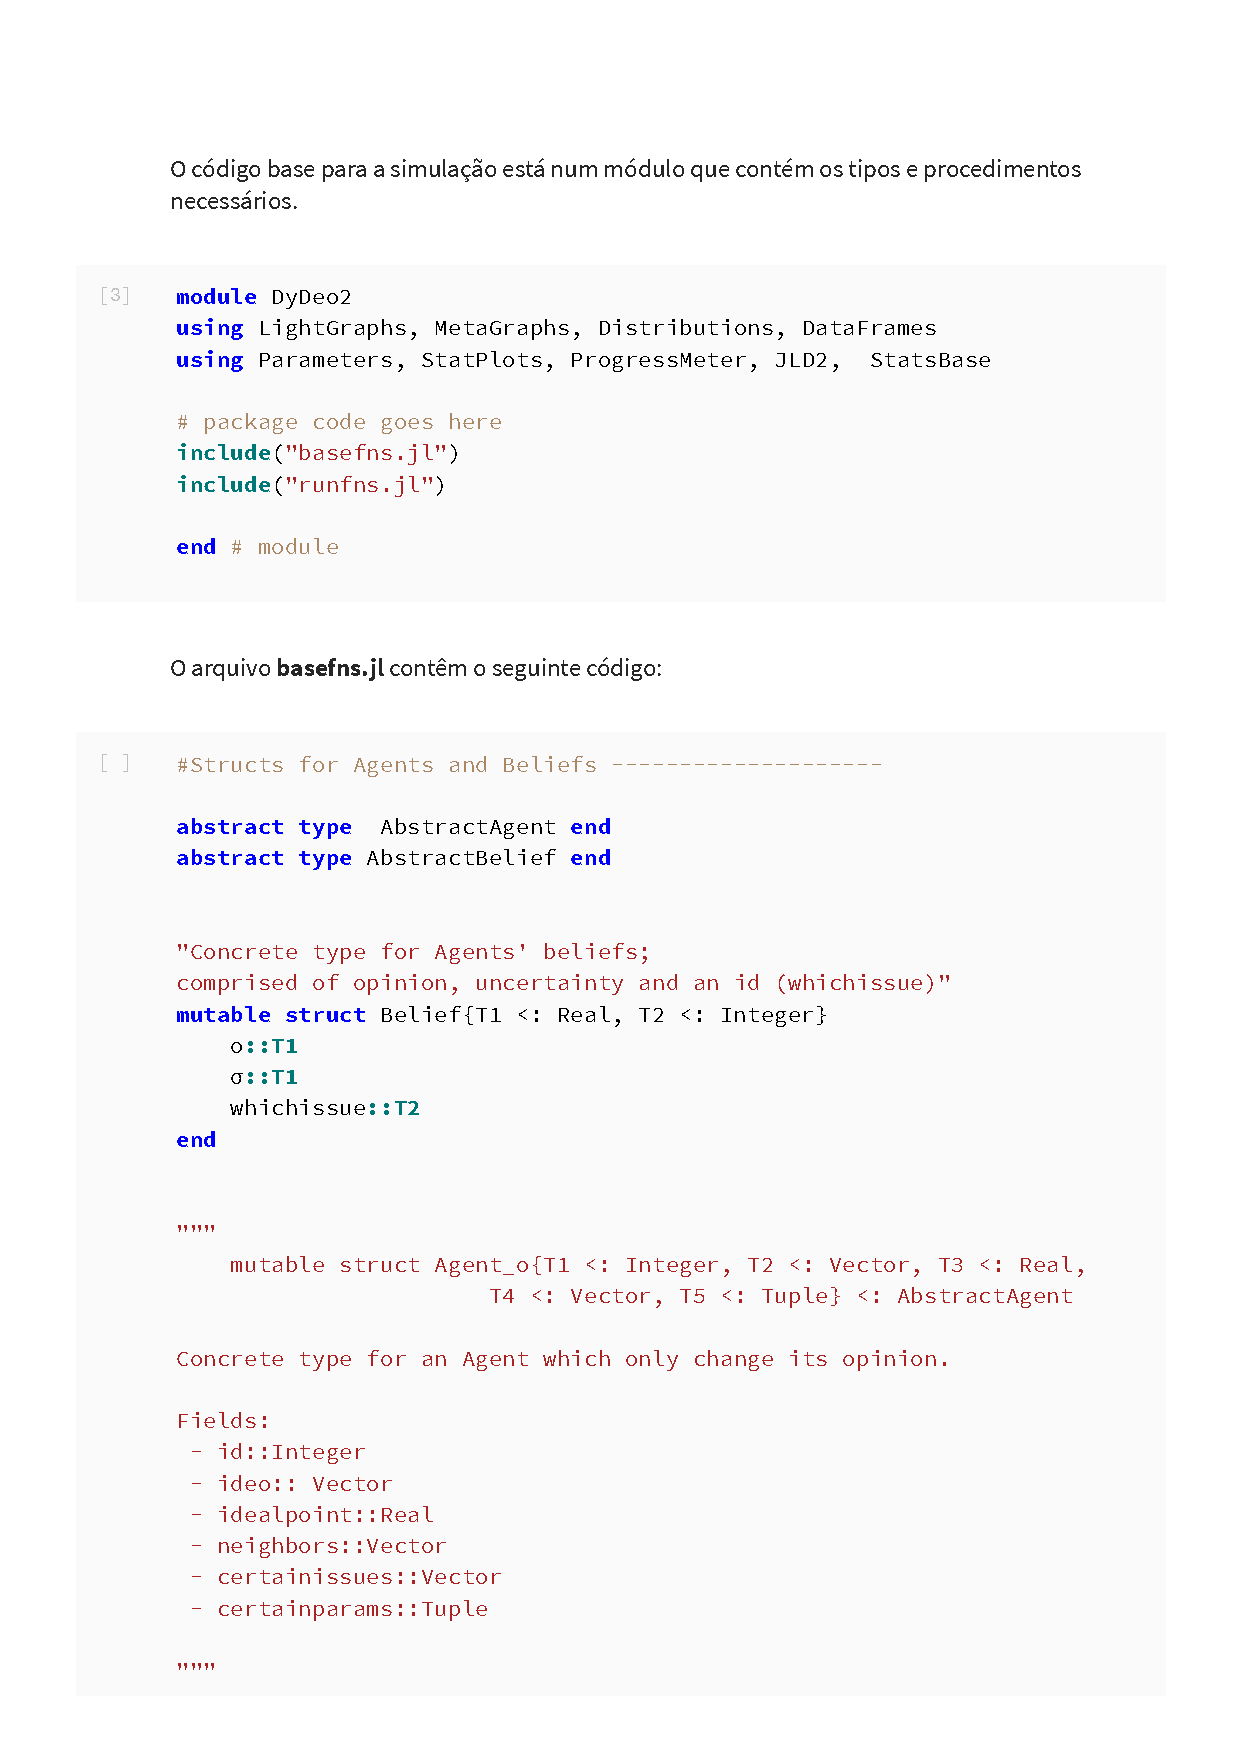
\includepdf[pages = {1,2,3,4,5,6,7,8,9,10,11,12,13,14}, pagecommand = {}, scale = 0.9]{ims/my-model.pdf}
